\clearpage
\section{WinResMon}
\label{sec:winresmon}

\mypreamble{
This section presents WinResMon, a resource usage monitoring framework for Windows.
The work was published in \cite{ramnath2006winresmon}.
After that, several enhancements have been implemented in order to support
our later work.
}

% \subsection{Introduction}

The tasks of software maintenance and configuration require a precise
understanding of system resources, the individual requirements of each piece
of software, and interdependencies between every software program on the
system.  We use the term {\em software maintenance} to describe the system
administration task of ensuring that software on a system is configured and
maintained correctly over time.  Examples of software dependencies include:

\begin{itemize}
\item File sharing: including dynamic libraries and external data storage.
\item Sharing of software configurations: usually in the form of registry keys
in Microsoft Windows.
\item Interprocess communication and synchronization.
\end{itemize}

Although software maintenance tasks might seem conceptually trivial, they can
be time consuming and difficult, especially in large or complex environments.
System administrators often rely on documentation and on-line information such
as FAQs or forums, but such information is often incomplete.

As discussed in Section~\ref{sec:wi-management},
in various distributions of Linux, software dependency issues are partly
addressed by the use of a package manager.  The Red Hat Package Manager (RPM)
\cite{ewing1996rpm}, for example, records the currently installed packages and the
files required and provided by these packages in a centralized database.  RPM
checks dependencies before removing a package to ensure that files required by
other installed packages are not removed.  Similar checks are done to prevent
installing a package which contains files that conflicts with other existing
packages.

In Microsoft Windows, however, software installation can be complex, and the
exact dependencies between different software programs might not be clear.
The confusion is further compounded by many implicit software
interdependencies, e.g. registry keys which are part of shared software
configurations.  As a result, it is difficult to know whether to remove a file
when uninstalling an application.  File removal might lead to problems with
another piece software or might create security vulnerabilities.  

When installing two or more programs that share files, one program may cease to
function correctly because the installation of the second blindly overwrote 
shared libraries (DLL files).  There is also the question of when to perform a
major software upgrade.  System administrators may delay upgrading
for fear of breaking existing software; yet such a choice has its own risks.

Our work focuses on the problem of software
maintenance in Microsoft Windows NT-based operating systems (e.g. Microsoft Windows
XP, Microsoft Windows 2000, Microsoft Windows 2003).\footnote{ While an
appropriate version of a tool similar to WinResMon could also be of use in UNIX,
its value is much greater in a Microsoft Windows environment.  } We present {\em WinResMon},
a discovery and system debugging tool for
determining a program's resource usage as well as the resource usage
interactions between multiple programs.
It is different from LBox as it provides whole system monitoring.

\subsection{Motivation and Applications}

We believe that the key to solving the software maintenance problem is to
understand the life cycle of the system and programs therein.  We also wish
to empower ordinary users, removing the requirement of knowing every minutiae
of Microsoft Windows.  Although WinResMon is not tailored specially for system
security, it can also be utilized as a security auditing tool.

We designed WinResMon to act as both an infrastructure or framework
and a system utility.  
As a framework, it is extensible, and one can therefore add
new functionality and build customized tools.  As a tool, it comes with
pre-built modules to answer typical questions about resource usage and
dependencies.

When used as a debugger, WinResMon investigates the current system state,
i.e. which program uses which registry keys, and determines how the system has
arrived at that state.  WinResMon accomplishes this by recording information
about the evolution of system software dependencies and resource usage over
time.  To solve general problems in software maintenance, WinResMon monitors:
files, the registry, and interprocess communication and synchronization.
However, it is not feasible to continuously and permanently record all changes
to the system since the required space would be prohibitive.  
WinResMon employs
a reasonable compromise by maintaining detailed usage records 
over the current time period and a
subset of information that can be maintained over the lifetime 
of all software in the system.

We illustrate the software maintenance problem with some simple examples.  One
attack vector for spyware is to register itself as a start-up program, thereby
hiding itself from the end user.  Also consider a music player which may
require some sound decoding libraries.  This application only functions
correctly with certain versions of the libraries.  Thus, replacing a library
can lead to software failure.  Various pieces of software may also conflict,
e.g.  two mail transfer agents (MTAs) usually do not co-exist.

Some common system administration questions and tasks which WinResMon 
can assist with include:

\begin{enumerate}

\item Can we safely remove a particular DLL file?

Some applications provide shared libraries (DLL files) for use with other
applications.  When the system administrator uninstalls an application, she
can also choose to remove the DLLs.  Removing a DLL can cause other programs
which still use it to malfunction.  On the other hand, blindly retaining all
DLLs will cause the system to keep growing and may create security
vulnerabilities.  The system administrator generally lacks adequate
information to determine whether another program uses a shared
library. WinResMon can be used to record the utilization of each DLL so that the
system administrator can determine which programs use which DLLs.

\item Why does a program need administrator privilege to run?

Running programs with administrator privilege is discouraged because malware
such as viruses/spyware or poorly written applications can damage the system.
However, some programs may need to run as the administrator without an obvious
reason.  WinResMon can detect whether a program needs administrator access.  The
idea is to understand the reasons for elevated privileges and configure the
system to limit the use of privileges.  If it finds applications that require
certain administrator privileges to function correctly, the system
administrator can set up a policy that restricts the administrator privileges
to the needed resources (files, registry keys, etc).  
We remark that this approach can be contrasted with confinement systems
such as systrace \cite{provos2003improving} in Unix.
WinResMon is an auditing tool, it does not confine system calls, but
provides useful input for system administrators to create policies 
on resource access which can then be used to limit privileges.

\item Monitoring sensitive registry locations to detect spyware.

Managing the Microsoft Windows registry is difficult due to its complexity.
Spyware often takes advantage of this complexity to bury itself in the
registry, making it difficult for the user to remove it completely.  In
\cite{wang2004gatekeeper}, the authors have listed the most common entry points for spyware
to enter a Windows NT system.  The following are some of the configuration
settings WinResMon can monitor:

\begin{itemize}

\item {\em Autostarts}: monitor which programs load on startup.
\item {\em Internet explorer hooks}: track hooks which define
the default search page, toolbars and browser helper objects (BHO), etc.
\item  {\em Winlogon}: look for applications that hook into system
resources.
\item  {\em Services}: monitor services such as automatic startup services
(e.g. task scheduler) or drivers which are installed as services.
\item {\em DLL injection}: monitor DLL injection attacks (any application
that uses {\small\tt user32.dll} can be hijacked by having a DLL injected into its
process space).
\item {\em File associations}: monitor the registration of file extensions
with applications.  For example, {\small\tt .DOC} is registered to Microsoft Word.

\end{itemize}
\end{enumerate}

\subsection{System Design}

The WinResMon system infrastructure shown in Figure~\ref{usp} consists of the
following components: logger, archiver, query API, and user-log API.  
The logger generates
resource-access traces which are later used by the analyzer.  The archiver
performs log compaction/summarization of old traces.
Query and user-log API provide the interface to the trace database.

\begin{figure*}
\centering
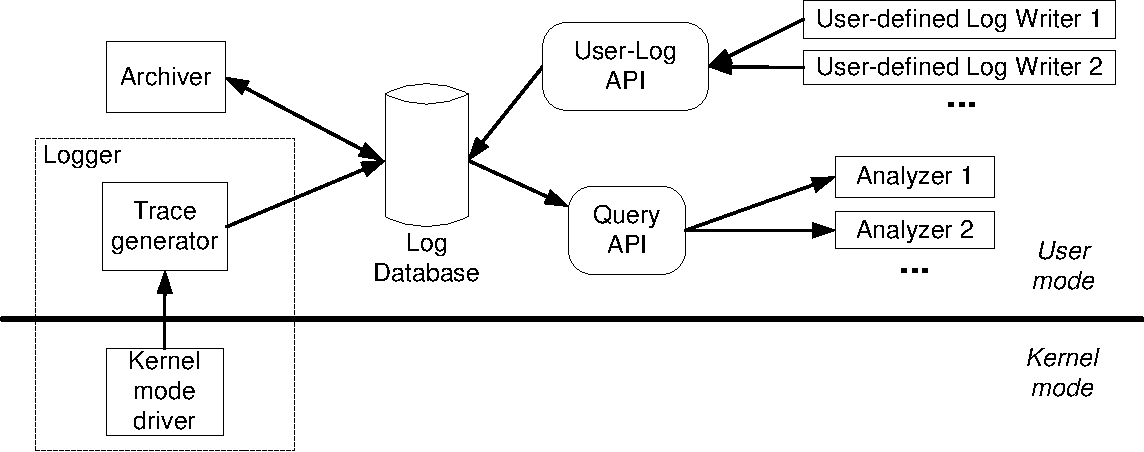
\includegraphics[scale=0.6]{winresmon/usp}
\caption{WinResMon overall system architecture}
\label{usp}
\end{figure*}


\subsubsection{The Logger}

The logger consists of a system call interceptor and a trace
generator module.  The system call interceptor is an in-kernel driver which
monitors system calls made by each process and sends the monitored event
information to the trace generator.  The trace generator is a user-space
service (daemon) which collects event information sent from the system call
interceptor and generates resource access traces.  Ideally, the logger is
meant to run {\em all the time} so as to record the entire life cycle of how
resources are used by software.\footnote{ One might only run the
logger at selected times instead, but this means WinResMon could miss critical information.}

A log trace file consists of a list of records, each representing 
an access operation on one of the following types of resource:

\begin{enumerate}
\item {\em File}: covering both directories and regular files
\item {\em Registry}
\item {\em Process}: mainly to record process creation
\item {\em Synchronization objects}: which records information on
inter-process synchronization mechanisms provided by Microsoft Windows (mutex,
semaphore, event and waitable timer)
\item {\em IPC}: including named pipes and mailslots.
\end{enumerate}

In addition to these five basic resource types, WinResMon also captures {\it
system event} information such as: process termination, system boot and
shutdown, user login and logout.  
Moreover, it also provides a user-log API
(described in Section~\ref{sect:custlog}) for users or applications to insert
user/application-defined milestone events.  One potential usage of custom
events is to demarcate and distinguish the software installation and
uninstallation portions of the log.

A record entry contains common information and specific information
relevant to that record type.
The common information consists of: {\em record-type}, 
{\em start-time}, {\em end-time}\footnote{
The timing is measured in CPU cycles, thus it is very accurate},
{\em process-id}, {\em thread-id}
{\em user-id} and the {\em error-code} 
(in the case of failure).  
We can optionally record the user space stack trace, which is a list
of function return addresses who directly or indirectly make the
system call.
This stack trace feature is used in our trace visualization (Sec.~\ref{sec:lviz}).
The specific information recorded by different record types are:

\begin{enumerate}
\item {\bf File:}
\begin{itemize}
\item absolute path of the file
\item file operation: {\em open}, {\em read}, {\em write}, {\em delete}
or {\em move}
\item operation-specific information. For open: the access flags.  For read
and write: the number of bytes read or written.  For move: the new path.
\end{itemize}

\item {\bf Registry:}
\begin{itemize}
\item absolute path of the registry key
\item operation:  {\em open-key}, {\em query-value}, {\em set-value}, or {\em
delete-key}
\item operation specific information.  For {\em open-key}: the access
flags. For {\em query-value} and {\em set-value}: the type, size, and value of
the registry key.
\end{itemize}

Due to the importance of the registry in software maintenance, WinResMon logs the
actual data changes made to the registry; whereas for file I/O, it is not
practical to record the data.

\item {\bf Process:}
\begin{itemize}
\item absolute path of the executable corresponding to the newly created
process
\item command line arguments
\item process id of the newly created process.
\end{itemize}

\item {\bf Synchronization objects:}
\begin{itemize}
\item type of the object:  {\em mutex}, {\em semaphore}, {\em event}, or
{\em waitable-timer}
\item name of the object
\item operation: {\em create}, {\em open}, or {\em delete}.
\end{itemize}

We are interested only in objects which have names in the system-wide
namespace, because anonymous and process-wide named objects will not interfere
with other programs, thus they are unrelated to software dependencies.

\item {\bf IPC:}
\begin{itemize}
\item type of the IPC: {\em named-pipe}, or {\em mailslot}
\item name of the IPC
\item operation: {\em create}, {\em open}, {\em delete}, {\em send}, or {\em
receive}. 
\end{itemize}

WinResMon records the synchronization objects and IPC operations listed above
since they involve global (system-wide) namespace which could
be used by different programs to interact with each other.
One can use WinResMon to uncover the causes of 
the following problems:

\begin{enumerate}

\item If process $A$ has created a semaphore $s$, and process $B$, which
is unaware of the existence of $A$, is trying to create a semaphore with the
same name $s$, $B$'s operation will fail.

\item If process $A$ fails to run correctly and semaphore $s$ is not
created, then process $B$, assuming the existence of $A$, will fail trying to
use $s$.
\end{enumerate}

\item {\bf System event:}
\begin{itemize}
\item system event type: {\em process-termination}, {\em boot}, {\em shutdown},
{\em user-login}, or {\em logout}
\item any event specific information: path of the executable of the process in
the case of process termination, user name in the case of user login/logout,
etc. 
\end{itemize}

\item {\bf User defined event:}
\begin{itemize}
\item the path of the executable of the process generating the event 
\item a binary string describing the event. 
\end{itemize}

\end{enumerate}

Not all operations need to be logged into the database as some resources are
not significant to record, e.g.  the temporary directory, {\tt
C:$\backslash$temp}.  A filter can therefore be used in the logger to prevent
logging resource access of no interest to the system administrator.


\subsubsection{The Log database}

The log database consists of a number of log files and one
distinguished {\it active log} to which the logger 
records current resource access activity.
To maintain reasonable log file sizes, WinResMon performs a ``log switch'' 
to create a new active log for recording subsequent entries.  The old
log files are then subject to the log compaction/summarization process by the
archiver.  Any of the following conditions can trigger a log switch: \\

\begin{itemize}
\item The size of the current log file reaches the specified {\tt
Max\_log\_size}.
\item The number of entries in the current log file reaches
{\tt Max\_log\_entries}.
\item The user manually initiates a log switch process.
\end{itemize}


\subsubsection{Archiving Old Traces}

As WinResMon logs system activities over a long period of time, the trace
becomes very large. If old traces are discarded, some early yet potentially valuable information,
such as identifying which program first created a file, is lost. An example of important information is
identifying which program first created a file.  Since it is necessary
to eventually prune some information to avoid excessively large log files,
WinResMon summarizes old trace files into a ``{\em compacted trace database}".
This maintains a balance between compactness and the ability to answer
important questions about system resource access.

There are two main issues in performing trace compaction, determining when to
initiate the compaction and how to perform compaction on old trace entries.
WinResMon uses a module called the archiver which runs based on a specified 
{\tt Archive\_interval\_check} time interval.  Upon activation, the archiver
compacts previously uncompacted entries which are older than the specified 
{\tt Old\_log\_age}.  
WinResMon employs the following strategies in performing the compaction:

\noindent
{\bf 1. Log entry summarization/aggregation}

WinResMon can summarize multiple entries with similar information to produce an
aggregated entry in the compacted trace database.  It applies the following
policies on various resource types:

\begin{itemize}

\item {\bf File:} multiple read or write operations on the same file are
summarized by recording the time of the first and last operations and the
total number of time the operations were done.

\item {\bf Registry:} multiple query-value operations on the same registry key
are aggregated.  Multiple set-value on a key are aggregated only if the values
written are identical.

\item {\bf IPC:} send and receive operations of one IPC object are aggregated
by recording the time of the first and last operations.

\end{itemize}

When matching a query (described later in Section~\ref{sect:queryapi})
on an aggregated entry which records a time interval,
WinResMon considers that the entry satisfies the specified time constraint
if {\it one} of the values matches the constraint.

\noindent
{\bf 2. Selective priority-based entry removal}

One strategy to reduce the old traces involves removing entries deemed to be
of little value for answering future questions. WinResMon implements selective
entry removal strategy based on a user-supplied configuration file.  The
configuration file assigns a priority to log entries.  For example, a log
entry for writing a registry key might be considered more important to keep
than one for reading a registry key.

A fragment of an example configuration is shown in Appendix 2.  This example
uses priority values ranging from 1 (least important) to 5 (most important).
For each resource type, configuration entries are matched in a sequential
order, and mappings are listed from most to least specific.  It is possible to
omit some arguments, i.e. with wildcards.  To simplify the priority
assignment, WinResMon classifies file open operations in Microsoft Windows 
into one of three modes: RO (read-only), RW (read-write) and WO
(write-only/append). The archiver translates the semantics of each operation
from file flags in the raw log entries to the appropriate values for matching
against the configuration.

The existing applications and anticipated usage, together with some general
principles, can be used to derive the priority assignment for the
configuration.  One general principle is that ``transient information,'' such as that
those on synchronization objects and IPC, becomes less relevant after
system shutdown and can be given low priority.  During the removal
process, all log entries with priority lower than the {\tt
Lowest\_priority\_retained} value will be purged.

\noindent
{\bf 3. Auto deletion of old log files}

To maintain reasonable storage usage, WinResMon eventually needs to remove
entries deemed too old.  The log file whose newest entry timestamp exceeds
{\tt Max\_log\_lifetime} is deleted.  If necessary, it is also possible to
additionally provide an API function (in a secure manner) to perform deletion
on selected trace entries based on a specified selection condition.


\subsubsection{A Query API and Analyzer}
\label{sect:queryapi}

We want to support trace analyzers which answer queries solving particular
software maintenance problems.  WinResMon therefore provides a query API which can be 
used to obtain information from the trace database.  
One can view the trace as a database and the provided query API as the query
language by which the analyzers extract relevant information from the
database.

The main query API, analogous to an SQL Select command, is
{\small\tt trace\_select([{\it selection condition}], [{\it field projection}],
[{\it time interval}], [{\it output order}])}, where the caller specifies
the matching condition(s) and fields to return.  The {\small\tt {\it selection
condition}}, specified on string types such as program name and registry key
path, takes the form of a regular expression.  Logical operators can be used
to combine matching conditions.

Continuing the database analogy, the caller uses projection to specify
which fields to return.  For example, suppose one only wants to know the list
of programs accessing a certain file.  In other cases, one wishes to know
all access operations on the file (i.e. the order and access time matter).
In the former, the analyzer only returns a set of program names.  In the
latter, it returns the sequence of all access operations.

We specify {\small\tt {\it time}} in the format below:
\begin{enumerate}
\item ``{\small\tt YYYY-MM-DD hh:mm:ss}'': an explicit timestamp
\item ``{\small\tt -[count][m|h|d]}'': a relative time earlier than the current time
\item ``{\small\tt OLDEST}'': the time of the oldest available entry in the log
\item ``{\small\tt NOW}'': the current time.
\end{enumerate}

The {\small\tt {\it time interval}} is then specified as: ``{\small\tt [{\it start time}] 
TO [{\it end time}]}''.\footnote{ Although an
analyzer can include constraints on log's timestamp as conditions in the
{\small\tt {\it selection condition}}, an explicit time interval specification is
less complex.  }
Some examples of time interval definitions are:

\begin{itemize}
\item ``{\small\tt 2006-01-25 11:47:51 TO 2006-08-21 13:41:16}''
\item ``{\small\tt -1d TO NOW}'' (in the last 24 hours)
\item ``{\small\tt OLDEST TO -8h}'' (everything except the past 8 hours).
\end{itemize}

{\small\tt {\it Output order}} controls the ordering of query results.  It can be
either: {\small\tt FORWARD}, to list the oldest entry first or {\small\tt BACKWARD}, to
show the most recent entry first.  The {\small\tt BACKWARD} option is useful to get
the $k$ most recent operations.

After obtaining the {\small\tt {\it trace\_handle}} from {\small\tt trace\_select()},
one can call {\small\tt trace\_next ({\it trace\_handle})} to retrieve the records
and {\small\tt trace\_close({\it trace\_handle})} to finish retrieval.
Some sample analyzer applications using this query API are described in
Section~\ref{sect:sample}.


\subsubsection{The User-Log API}
\label{sect:custlog}

The user-log API lets applications add their own entries into the log
database.  As applications are not allowed to write directly to the log file,
custom events are generated using an {\small\tt ioctl} interface to the kernel
driver.  One use of user-entries includes marking events related to software
installation, making it easier to determine what files and registry keys are
created/modified during installation.  This feature also provides a general
purpose logging facility.

The API for user-entries is {\small\tt winresmon\_userlog({\it logdata}, {\it
length})}.  It signals the trace generator to record the {\small\tt {\it logdata}}
to the log database in binary form.  The ownership information of a user log
entry (i.e. the program pathname and process) is always recorded.

Figure~\ref{custlog-prog} shows a simple wrapper for an installer program which
generates custom installation events.  In this example, the {\small\tt {\it
logdata}} consists of the name of the software and path of the installer
program.  Invoking the wrapper as ``{\small\tt C:$\backslash$ins-wrapper.exe
photoshop\_cs2 H:$\backslash$setup.exe}'', generates {\small\tt {\it logdata}}
containing ``{\small\tt INBGH:$\backslash$setup.exe|photoshop\_cs2}'' and
``{\small\tt INEDH:$\backslash$setup.exe|photoshop\_cs2}''.

\begin{figure}[htb]
\hrule
\medskip
\small
\begin{verbatim}
#define MAGIC_INSTALL_BEGIN "INBG"
#define MAGIC_INSTALL_END   "INED"

int main (int argc, char **argv)
{
  char buff[256];

  if (argc != 3) {
    printf("example: %s software_name c:\...\installer.exe", argv[0]);
    exit(1);
  }

  buff[sizeof(buff)-1] = '\0';
  _snprintf(buff, sizeof(buff)-1, MAGIC_INSTALL_BEGIN "%s|%s",
      argv[2], argv[1]);
  winresmon_userlog(buff, strlen(buff));
  system(argv[2]); // fork and wait
  _snprintf(buff, sizeof(buff)-1, MAGIC_INSTALL_END "%s|%s",
      argv[2], argv[1]);
  winresmon_userlog(buff, strlen(buff));
  return 0;
}
\end{verbatim}
\hrule
\medskip
\caption{A sample installer wrapper}
\label{custlog-prog}
\end{figure}


\subsection{Implementation}

\begin{figure}[htb]
\centering
\begin{picture}(240,150)
\thinlines
\put(38,96){\framebox(70,15){iexplore.exe}}
\put(121,96){\framebox(80,15){trace generator}}
\put(50,6){\framebox(129,16){syscall dispatcher}}
\put(50,42){\framebox(129,16){syscall interceptor}}
\put(126,129){\framebox(61,14){trace file}}
\put(8,75){\line(220,0){220}}
\put(63,96){\vector(0,-38){38}}
\put(87,42){\vector(0,-20){20}}
\put(97,22){\vector(0,20){20}}
\put(161,58){\vector(0,38){38}}
\put(75,58){\vector(0,38){38}}
\put(161,111){\vector(0,18){18}}
\put(208,82){user}
\put(200,62){kernel}
\put(0,80){1. CreateFile()}
\put(20,28){2. pass down}
\put(100,28){3. return}
\put(138,80){4. send event}
\put(166,116){5. log}
\put(76,80){6. return}
\end{picture}
\caption{Overview of how the logger works}
\label{logger}
\end{figure}

Figure~\ref{logger} gives an overview of how the logger works.
The information flow is as follows:

\begin{enumerate}
\item A sample program {\small\tt iexplore.exe} calls
{\small\tt CreateFile("\path{C:\WINDOWS\system32\Macromed\Flash\Flash8.ocx}", READ, ...)}.
\item This is intercepted by our system call interceptor
which passes the parameters to the original system call handling routine.
\item The system call handling routine returns the file handle.
\item The handle, together with the system call parameters are then sent to
the trace generator.
\item As the call is successful, the trace generator updates 
the file handle/path lookup table.
Since {\small\tt "foo"} is a relative path, the trace generator concatenates
{\small\tt "foo"} with the current directory and add it to the trace.
\item The handle is returned to {\small\tt iexplore.exe} and operation
continues as per normal.\footnote{Step 6 and 4 are independent.
Thus, depending on the scheduler, step 6 is not necessarily executed after
x
step 4.} 
\end{enumerate}


\subsubsection{System call interception}

The overview of the logger in Figure~\ref{logger} shows that resource usage is
captured by intercepting system calls.
\TODO{de-repetation}
As discussed in Section~\ref{sec:bg-win}, this is actually more complex.
Rather than defining and using the actual system calls, the
Microsoft Windows API is described at a level higher than the operating system
using the Win32 API.  Although most programs use Win32, they can use the
native API \cite{nebbett2000windows} directly.  The native system call interface API
is unfortunately not well documented and supported.  Furthermore, the view of
the operating system at the native API level is not quite the same as at the
Win32 level.  This means that intercepting system calls at what regular
programs might think of as the Microsoft Windows API is problematic, and there
could be discrepancies and mismatches between API use at the Win32 level and
native level.  To ensure accuracy, WinResMon intercepts system calls at the
native API level.

WinResMon implements the system call interceptor by means of a kernel mode driver.
The driver captures system call requests made by a process by ``hooking'' the
native system calls as described in \cite{ddj-nthooking}.  Appendix 1 lists the
system calls intercepted by WinResMon.  We found these to be the most common
system calls arising from file, registry, IPC, synchronization, and process
operations.\footnote{ Since Microsoft Windows is closed source and the native
API is only partially documented, it is difficult to make any guarantees about
completeness.  }

To gather information about processes, WinResMon uses a simpler method.
Microsoft Windows NT exports a set of process callback functions in the kernel
space \cite{msdn-proccallback}.
WinResMon makes use of {\small\tt PsSetCreateProcessNotifyRoutine()} and
{\small\tt PsSetLoadImageNotifyRoutine()} which notifies the call back function
during process creation or termination.


\subsubsection{Event handling}

When sending the data from the kernel to the user space, it is inefficient to
send every event as it arrives.  WinResMon's implementation therefore makes use
of double buffering.  When the size of a buffer reaches a threshold, WinResMon
sends the contents of the buffer to the user space and switches to another
buffer to continue logging in the kernel space.  This strategy tries to ensure
that most, if not all, events are captured and reduces the system overhead due
to context switching.  Again, due to the undocumented nature of the kernel, we
cannot claim to capture all events.

In the prototype implementation, the kernel and user space communicate through
an ioctl mechanism. Ioctls are used to define a protocol 
to synchronize data transfer between the driver and 
user level trace generator.
WinResMon can also be extended to as a remote-monitoring tool.


\subsection{Writing Custom Analyzers}
\label{sect:sample}

This section demonstrates how to write custom analyzers on top of the WinResMon
framework by means of examples.

\begin{itemize}

\item An analyzer to show all the programs which read {\tt
C:$\backslash$foo.txt} after 2005/1/1 could use the following
query:

{\small\tt \begin{tabbing}
trace\_\=select \kill
trace\_select("file.path == $\backslash$"C:$\backslash\backslash$foo.txt$\backslash$"", \\
	\>"prog\_path", \\
	\>"2005-1-1 00:00:00 TO NOW", \\
	\>FORWARD);.
\end{tabbing}}

\item A more complicated example asks, ``What's the most recent execution of
{\tt msnmsgr.exe} before this boot?''  First determine the last {\it
shutdown\_time} with the query:

{\small\tt \begin{tabbing}
trace\_\=select \kill
trace\_select("sysevent.type == $\backslash$"shutdown$\backslash$"", \\
	\>"time", \\
	\>"OLDEST TO NOW", \\
	\>BACKWARD);
\end{tabbing}}

The next query gets the whole process creation event
for {\small\tt msnmsgr.exe}: 

{\small\tt \begin{tabbing}
trace\_\=select \kill
trace\_select("proc.childname =\~{} \\
	\>$\backslash$"/\^{}.*$\backslash\backslash$msnmsgr.exe\$/$\backslash$"", \\
	\>NULL, \\
	\>"OLDEST TO {\it last\_shutdown\_time}", \\
	\>BACKWARD);
\end{tabbing}}

\item Figure~\ref{analyzer-prog} shows a code fragment from a simple analyzer
which searches for all the registry keys opened by Internet Explorer.

\begin{figure}[htb]
\small
\hrule
\medskip
\begin{verbatim}
struct trace_struct *handle;
struct trace_entry *entry;

trace_handle = trace_select(
    "type==\"registry\" && "
    "prog_path=~\"/iexplorer.exe$/\"",
    "time, registry.path",
    "-1d TO NOW",
    FORWARD);
if (trace_handle == NULL)
   exit(1);
while ((entry = trace_next(trace_handle)) != NULL) {
  printf("time=%s, registry=%s",
      entry->fields[0], entry->fields[1]);
}
trace_close(trace_handle);
\end{verbatim}
\hrule
\caption{A sample analyzer}
\label{analyzer-prog}
\end{figure}

\noindent

WinResMon issues the query with selection {\small\tt type == "registry" \&\&
prog\_path =\~{} "/iexplorer.exe\$/"} and projection on {\small\tt time} and
{\small\tt registry.path}.  After correctly obtaining a {\small\tt trace\_handle}, it
iterates over all selected records by using {\small\tt trace\_next()}.  It prints
all the fields, {\small\tt time} and {\small\tt registry.path}, for each selected trace
entry.  After iterating over all relevant records, it closes the handle.

\end{itemize}


\subsection{Using WinResMon}

The extended example below shows the use of WinResMon to solve software
maintenance problems.

Yahoo Toolbar adds tabbed browsing to Internet Explorer (IE) and
adds various icons and links from within IE to different Yahoo services.  The
following walk-through illustrates monitoring the Yahoo toolbar throughout its
entire life cycle.  There are three stages:

\begin{enumerate}
\item Installation

The provided installer refuses to run under a standard user account as it
needs administrator privileges. Upon successful installation under an
administrator account, it creates the following DLLs and keys:

\noindent DLLs:\\
\path{C:\Program Files\Yahoo!\Companion\Installs\cpn\yt.dll}\\
\path{C:\Program Files\Yahoo!\Companion\Installs\cpn\YTabBar.dll}\\
\path{...}

\noindent Registry keys:\\
\path{HKEY\_LOCAL\_MACHINE\SOFTWARE\Yahoo}

 From our list of sensitive registry locations, we note the following.

\noindent Before Installation: \\
Search Page: \\
\url{http://www.microsoft.com/isapi/redir.dll?prd=ie&ar=iesearch} \\
Search Bar:  -

\noindent After Installation: \\
Search Page: \\
\url{http://us.rd.yahoo.com/customize/ycomp/defaults/sp/*http://www.yahoo.com} \\
Search Bar: \\
\url{http://us.rd.yahoo.com/customize/ycomp/defaults/sb/*http://www.yahoo.com/search/ie.html} \\
Yahoo! Toolbar Helper: \\
\path{02478D38-C3F9-4EFB-9B51-7695ECA05670} -
\path{C:\Program Files\Yahoo!\Companion\Installs\cpn0\yt.dll}

Among the changes made, Yahoo replaced MSN search as the default search
engine.

\item Program usage

Since the database is persistent, WinResMon logs all the events associated with
Yahoo and preserves the information even if the system reboots.  This helps
analyze the behavior of Yahoo toolbar over a period of time.

\item Uninstalling

When uninstalling Yahoo toolbar, WinResMon observes that all the files have been
removed.  However, the registry settings it made are left unchanged. As a
result, Yahoo remains the default search engine for the system.

\end{enumerate}


\subsection{WinResMon Overhead}
\label{sec:resmon-overhead}

To measure the performance overhead resulting from constant
monitoring of systems with WinResMon,  we first look at some
worst case scenarios using micro-benchmarks consisting of only
repeated system calls.

Our micro-benchmarks comprise of: seven benchmarks on file access, five on registry access, and
two on process creation.  All of these micro-benchmarks run on a
Pentium 4 2.4GHz machine with 512MB running Microsoft Windows XP with SP2.
The benchmarking procedure consists of first running the benchmarks on a 
clean Microsoft Windows XP (with SP2) to get the baseline performance.
We then run with WinResMon loaded.
Finally, we run with FileMon~\cite{filemon} loaded for file access
benchmarks and RegMon~\cite{regmon} loaded for registry access benchmarks.
Each micro-benchmark repeats an operation $n$ times.
We performed each benchmark four times to get the average execution time.
Table \ref{tab:winresmon-perf-fr} and \ref{perf-proc} show the average and standard 
deviation of the execution time in seconds.

The file access benchmarks consist of:

\begin{description}
\item[$(F_1)$] Open an existing file.  The same filename is used every time.
\item[$(F_2)$] Create a new file and delete it.  A different filename is used
every time. 
\item[$(F_3)$] Read 1 byte from a file. We ensure that the file is large
enough so that EOF is never met for multiple reads.
\item[$(F_4)$] Read 4,096 bytes from a file.  The file size is a multiple of
4,096. When we reach EOF, we rewind to the beginning of the file.
\item[$(F_5)$] Write 1 byte to a file.  We start with an empty file.
\item[$(F_6)$] Write 4,096 bytes to a file.  When we reach EOF, we rewind to
the beginning of the file. 
\item[$(F_7)$] Create a new directory and delete it. A different filename is
used every time. 
\end{description}

The benchmarks for registry access are:

\begin{description}
\item[$(R_1)$] Open an existing registry key.  The same key is used every time.
\item[$(R_2)$] Create a new registry key and delete it.  A different name is
used every time. 
\item[$(R_3)$] Create a new volatile registry key and delete it.
{\small\tt RegCreateKeyEx} is used with the {\small\tt REG\_OPTION\_VOLATILE} option.
\item[$(R_4)$] Query the value of a registry key.  The type {\small\tt REG\_DWORD}
is used. 
\item[$(R_5)$] Set the value of a registry key.  The type {\small\tt REG\_DWORD} is
used. 
\end{description}

The benchmarks for process creation are:

\begin{description}
\item[$(P_1)$] Create a dummy console process and wait for its termination.
\item[$(P_2)$] Create a dummy GUI process and wait for its termination.
\end{description}

\begin{sidewaystable*}
\centering
\begin{tabular}{|l|l|c|c|c|}
\hline
File Operation & $n$ & Clean & WinResMon & FileMon \\
\hline
($F_1$) Open an existing file  & 1M   & $20.457 \pm 0.240$  & $46.266 \pm 3.271$ ($126.2\%$)    & $44.168 \pm 0.279$ ($116.0\%$)\\
($F_2$) Create a new file      & 100K & $53.004 \pm 2.532$  & $67.539 \pm 0.469$ ($27.4\%$)     & $73.117 \pm 0.265$ ($37.9\%$) \\
($F_3$) Read 1 byte            & 10M  & $14.277 \pm 1.084$  & $278.175 \pm 14.282$ ($1848.4\%$) & $107.414 \pm 4.765$ ($652.4\%$) \\
($F_4$) Read 4096 bytes        & 10M  & $41.207 \pm 0.133$  & $328.203 \pm 34.869$ ($696.5\%$)  & $138.816 \pm 0.793$ ($236.9\%$) \\
($F_5$) Write 1 byte           & 10M  & $49.824 \pm 1.160$  & $388.050 \pm 0.837$ ($678.8\%$)   & $172.422 \pm 1.114$ ($246.1\%$) \\
($F_6$) Write 4096 bytes       & 10M  & $116.355 \pm 0.716$ & $448.933 \pm 2.192$ ($285.8\%$)   & $212.828 \pm 2.950$ ($82.9\%$) \\
($F_7$) Create a new directory & 100K & $46.546 \pm 0.344$  & $57.750 \pm 9.565$ ($24.1\%$)     & $56.395 \pm 0.282$ ($21.2\%$) \\
\hline
\hline
Registry Operation & $n$ & Clean & WinResMon & RegMon \\
\hline
($R_1$) Open an existing key  & 1M   & $10.378 \pm 0.039$ & $35.324 \pm 0.080$ ($240.4\%$)  & $361.438 \pm 40.504$ ($3382.7\%$) \\
($R_2$) Create a new key      & 100K & $8.980 \pm 0.037$  & $13.769 \pm 0.041$ ($53.3\%$)   & $134.879 \pm 10.778$ ($1402.0\%$) \\
($R_3$) Create a new temp key & 100K & $7.832 \pm 0.045$  & $12.750 \pm 0.082$ ($62.8\%$)   & $142.961 \pm 12.811$ ($1725.3\%$) \\
($R_4$) Query value           & 1M   & $1.461 \pm 0.009$  & $27.203 \pm 0.061$ ($1761.9\%$) & $166.301 \pm 4.406$ ($11382.7\%$) \\
($R_5$) Set value             & 1M   & $22.890 \pm 0.153$ & $46.379 \pm 0.090$ ($102.6\%$)  & $182.473 \pm 7.272$ ($697.1\%$) \\
\hline
\end{tabular}
\caption{Performance comparison on file and registry access ($n$ operations in seconds)}
\label{tab:winresmon-perf-fr}
\end{sidewaystable*}

Table~\ref{tab:winresmon-perf-fr} shows the execution time (in seconds)
for the file and registry access benchmarks.
In order to avoid any extraneous overhead from the FileMon and RegMon
GUI, the window is always minimized during the experiments.
It appears that both FileMon and RegMon do not capture all the operations
during the performed micro-benchmark, though.
For example, during the ``Read 1 byte'' test, 10M
events occurred, but FileMon only captured about 15K.
During the ``Create a new file'' test, 600K events occurred,
but only about 18K were actually captured.
During the ``Query value'' test, 1M events occurred, but only 993,938
were actually captured by RegMon.
We observe that WinResMon, by contrast, captured all
operations in all the tests.

Note that FileMon, RegMon and WinResMon address different goals.
FileMon and RegMon are meant for short term monitoring while WinResMon is
designed for long term use and is therefore always running in the background.
These two benchmark comparisons merely give us a baseline on how WinResMon
compares with other, similar monitoring software.

\begin{table*}
\small
\centering
\begin{tabular}{|l|l|c|c|}
\hline
Process Operation & $n$ & Clean & WinResMon \\
\hline
($P_1$) Create a console process & 10K & $35.488 \pm 0.071$ & $37.855 \pm 0.150$ ($6.7\%$) \\
($P_2$) Create a GUI process     & 10K & $34.641 \pm 0.044$ & $36.938 \pm 0.097$ ($6.7\%$) \\
\hline
\end{tabular}
\caption{Performance of process creation (in seconds)}
\label{perf-proc}
\end{table*}

\begin{table*}
\small
\centering
\begin{tabular}{|l|c|c|}
\hline
Test Case & Clean & WinResMon \\
\hline
WinRAR   & $224.443 \pm 0.542$ & $226.524 \pm 3.502$ ($0.9\%$) \\
gcc      & $26.265 \pm 1.219$  & $26.973 \pm 0.968$ ($2.70\%$) \\
\LaTeX{} & $27.211 \pm 0.473$  & $27.498 \pm 0.981$ ($1.1\%$) \\
Lame     & $45.631 \pm 0.538$  & $45.662 \pm 0.534$ ($0.6\%$) \\
\hline
\end{tabular}
\caption{Performance of macro-benchmarks (in seconds)}
\label{perf-macro}
\end{table*}

Table~\ref{perf-proc} shows the results of the process creation benchmark. The
console process in the benchmark creates a dummy child process using the
{\small\tt CreateProcess()} function and waits for its termination using the
{\small\tt WaitForSingleObject()} function.  The difference between a console
program and a GUI program is that the GUI program uses the {\small\tt WinMain()}
entry function and is linked using the {\small\tt /SUBSYSTEM:WINDOWS} option, while
the console program uses {\small\tt main()} and {\small\tt /SUBSYSTEM:CONSOLE}.  The
measured overhead is quite small because process creation is a slower
operation than file or registry access.

We would expect normal programs to have much smaller overhead than that of the
micro-benchmarks because the micro-benchmarks are very system call intensive.
Normal programs, such as our macro-benchmarks, typically make significantly
fewer system calls, spending more time in the application rather than the
kernel.
Table~\ref{perf-macro} gives some macro-benchmark results which show the
impact of WinResMon on the following normal programs: {\small\tt WinRAR}, {\small\tt gcc}, \LaTeX{} and {\small\tt Lame}.
The benchmarks perform the following:
\begin{itemize}
\item {\small\tt WinRAR}: compress a 150MB file.  
\item {\small\tt gcc}: compile a 500K-line C program.  
\item {\small\tt latex}: compile a 2,000-page \LaTeX{} file into PDF using the
{\small\tt pdflatex} program.
\item {\small\tt Lame}: encode a 100M wave file into a mp3 file. 
\end{itemize}
The macro-benchmark results demonstrate that running WinResMon all the 
time  is quite reasonable under typical usage.


\subsection{Related Work}

 From a high level perspective, WinResMon differs from previous systems/tools in
that it is:

\begin{itemize}
\item {\em integrated}: since it monitors accesses on files and registry
under one infrastructure
\item {\em extensible}: system administrators can write their own custom
modules to utilize the generated log
\item {\em geared for log management}: system administrators can view
resource access activities generated over time, and inspect their relationships
with respect to software configuration and dependencies.
\end{itemize}

We briefly mention some other tools/systems below, and highlight the important
differences with WinResMon.

WinResMon shares the basic monitoring functionalities with
FileMon and RegMon tools (Sec.~\ref{sec:sysinternals}).
However, WinResMon's
infrastructure is integrated, and its log database is designed to assist
system administrators in inspecting software configuration and dependencies.

Strace (Sec.~\ref{sec:ptrace}) is a Linux/UNIX tool used to intercept and log system
calls invoked by a process.  There is also a Microsoft Windows NT port of
strace with similar functionality.  WinResMon differs from
strace in that is focused more on resource usage (files, registry, etc) rather
than system calls.  In Windows, a system call viewpoint can be
confusing since there are multiple levels of APIs which translate into the poorly
documented native API.

Systrace \cite{provos2003improving} is a UNIX tool for sandboxing untrusted code.  Unlike
Systrace, which examines system-call sequences issued by the monitored
processes and applies a specific security policy, WinResMon is meant as a
monitoring tool to inspect resource usage and interactions among programs in a
system.

DTrace (Sec.~\ref{sec:dtrace}),
SystemTap (Sec.~\ref{sec:systemtap}) and
LBox (Sec.~\ref{sec:lbox}) are
auditing and instrumentation systems on various UNIX operating systems.  They
are all event based auditing systems, performing a specific action only on a
specific event.  DTrace and SystemTap allow administrators to dynamically
execute supplied code in the kernel when certain event occurs.  LBox allows
the kernel to notify a user space program when certain events happen.  Both
LBox and WinResMon are designed for monitoring resource usage, while DTrace and
SystemTap are designed for general system call instrumentation.


\subsection{Conclusion}

We presented the motivation, design, implementation and usage of
WinResMon.  Its main use is to inspect resource access and software dependency
issues in Microsoft Windows environments.  As WinResMon is extensible, system
administrators can also build tools using WinResMon for custom queries and
system analysis.  Benchmarking shows that WinResMon is reliable and is
comparable to other popular tools.

Future work is to increase the usability and robustness.
We would also like to ensure that logging is as comprehensive as possible
taking into account the undocumented
and unsupported nature of the APIs in the Microsoft Windows NT kernel.
We would also like to further increase the efficiency of the
logging mechanism.

In Chapter~\ref{sec:vis}, we will show how WinResMon's log can be explored
through visualization.
While we have shown how our query API can be used to answer software
dependency questions,
in Section~\ref{sec:depvis}, we will show how we can visualize
a particular type of dependency --- module dependency.
WinResMon's log not only can be considered as a database recording
the program-resource relation, but also can be considered as a trace
recording program behaviours.
In Section~\ref{sec:lviz}, we will visualize WinResMon's log in order
to study program behaviours, including repeated patterns, abnormal events
and behaviour differences,
which are useful to discover various of problems.

% \begin{thebibliography}{99}
% 
% \bibitem{rpm}
% \url{http://www.rpm.org/}.
% 
% \bibitem{systrace}
% N. Provos, ``Improving Host Security with System Call Policies'', USENIX
% Security Symposium, pp. 257--272, 2003. 
% 
% \bibitem{asep}
% Y. M. Wang, R. Roussev, C. Verbowski, A. Johnson, M. W. Wu,
% Y. Huang and S. Y. Kuo,
% ``Gatekeeper: Monitoring Auto-Start Extensibility Points
% (ASEPs) for Spyware Management'',
% Large Installation System Administration Conference, pp. 33--46, 2004.
% 
% \bibitem{ntnativeapi}
% G. Nebbett, ``Windows NT/2000 Native API Reference'', Macmillan Technical
% Publishing, Indianapolis, 2000. 
% 
% \bibitem{nthooking}
% \url{http://www.ddj.com/184410109}.
% 
% \bibitem{MSDN}
% Microsoft MSDN, ``Process Callbacks",
% \url{http://msdn.microsoft.com/library/default.asp?url=/library/en-us/Kernel_r/hh/Kernel_r/k108_a0f7bff2-270e-41fb-87d4-d8d533aa0bef.xml.asp}.
% 
% \bibitem{yahoo}
% \url{http://toolbar.yahoo.com/}.
% 
% \bibitem{filemon}
% \url{http://www.sysinternals.com/Utilities/Filemon.html}.
% 
% \bibitem{regmon}
% \url{http://www.sysinternals.com/Utilities/Regmon.html}.
% 
% \bibitem{strace}
% \url{http://www.liacs.nl/~wichert/strace/}.
% 
% \bibitem{bindview}
% \url{http://www.bindview.com/Services/RAZOR/Utilities/Windows/strace_readme.cfm}.
% 
% \bibitem{dtrace}
% B. M. Cantrill, M. W. Shapiro and A. H. Leventhal, ``Dynamic Instrumentation of
% Production Systems'', USENIX Annual Technical Conference, pp. 15--28, 2004.
% 
% \bibitem{systemtap}
% V. Prasad, W. Cohen, F. Eigler, M. Hunt, J. Keniston, B. Chen, ``Locating
% System Problems Using Dynamic Instrumentation'', Linux Symposium, vol. 2,
% pp. 57--72, 2005. 
% 
% \bibitem{lbox}
% Y. Z. Wu and R. H. C. Yap, ``A User-level Framework for Auditing and
% Monitoring'', Annual Computer Security Applications Conference, pp. 95--105, 2005.
% 
% \end{thebibliography}
% 
% \newpage
% \onecolumn
% 
% 
% \section*{Appendix 1: List of Intercepted System Calls}
% 
% Table~\ref{loggedcalls} lists the Microsoft Windows NT native-level system
% calls intercepted in our current implementation.
% 
% \begin{table}[here]
% \centering
% \begin{tabular}{|l|l|}
% \hline
% \multicolumn{2}{|c|}{File} \\
% \hline
% ZwCreateFile & opens or creates a new file \\
% ZwOpenFile & opens an existing file \\
% ZwDeleteFile & deletes a file \\
% ZwReadFile & reads from an open file \\
% ZwWriteFile & writes to an open file \\
% ZwQuerySystemInformation & queries for information internal to the system \\
% \hline
% \multicolumn{2}{|c|}{Registry} \\
% \hline
% ZwCreateKey & opens an existing key or creates it if it does not exist \\
% ZwDeleteKey & deletes a key \\
% ZwOpenKey & opens an existing key \\
% ZwQueryKey & provides information about the size and number of subkeys (if
% any) \\ 
% ZwQueryValueKey & provides the value of a registry key entry \\
% ZwSetValuekey & creates or replaces a registry key's value entry \\
% ZwDeleteValueKey & deletes a registry key's value entry \\
% \hline
% \multicolumn{2}{|c|}{Process} \\
% \hline
% ZwTerminateProcess & terminates a process and all its threads. \\
% \hline
% \multicolumn{2}{|c|}{Synchronization Object (Mutex)} \\
% \hline
% ZwCreateMutant & creates a mutex or opens an existing mutex \\
% ZwOpenMutant & opens an existing mutex \\
% \hline
% \multicolumn{2}{|c|}{Synchronization Object (Semaphore)} \\
% \hline
% ZwCreateSemaphore & creates a semaphore or opens an existing semaphore \\
% ZwOpenSemaphore & opens an existing semaphore \\
% \hline
% \multicolumn{2}{|c|}{Synchronization Object (Event)} \\
% \hline
% ZwCreateEvent & creates a new event or opens an existing event \\
% ZwOpenEvent & opens an existing event \\
% \hline
% \multicolumn{2}{|c|}{Synchronization Object (Waitable Timer)} \\
% \hline
% ZwCreateTimer & creates a new timer object or opens an existing timer object \\
% ZwOpenTimer & opens an existing timer object \\
% \hline
% \multicolumn{2}{|c|}{IPC (Named pipe)} \\
% \hline
% ZwCreateNamedPipeFile & creates a named pipe \\
% \hline
% \multicolumn{2}{|c|}{IPC (Mailslot)} \\
% \hline
% ZwCreateMailslotFile & creates a mailslot \\
% \hline
% \end{tabular}
% \caption{Intercepted system calls}
% \label{loggedcalls}
% \end{table}
% 
% 
% \section*{Appendix 2: Example of Log Priorities for Trace Compaction}
% 
% The following example shows a fragment from a log configuration which assigns
% priorities on FILE resource-type entries.  We map log entries into priority
% values ranging from 1 (least important to retain) to 5 (most important to
% retain).
% 
% \medskip
% \hrule
% \begin{small}
% \begin{verbatim}
% # File Section
% # Format:
% # Type	 Action  Object                                      Mode    Priority
% FILE    Read    *                                            *         1
% FILE    Write   *                                            *         1
% File    Open    C:\Windows\Temp\*                            *         1
% File    Open    C:\Windows\System32\*                        RW|WO     5
% File    Open    C:\Windows\System32\*                        RO        4
% File    Open    C:\Windows\*                                 RW|WO     4
% File    Open    C:\Windows\*                                 RO        3
% File    Open    C:\Program Files\*                           RW|WO     3
% File    Open    C:\Program Files\*                           RO        2
% File    Open    C:\Documents and Settings\Local Settings\
%                 {Temp\*|Temporary Internet Files\*}	         *         1
% File    Open    *                                            RW|WO     2
% File    Open    *                                            RO        1
% File    Delete  C:\Windows\Temp\*                            *         1
% File    Delete  C:\Windows\System32\*                        *         5
% File    Delete  C:\Windows\*                                 *         4
% File    Delete  C:\Program Files\*                           *         3
% File    Delete  C:\Documents and Settings\Local Settings\
%                 {Temp\*|Temporary Internet Files\*}          *         1
% File    Delete  *                                            *         2
% .... 
% \end{verbatim}
% \end{small}
% \hrule
% 
% \end{document}
